\chapter{cta}
\label{cta}


\section{A short history of ground-based atmospheric cherenkov atronomy}
In the time between the discovery of cosmic radiation by Victor Hess \cite{Hess:1912srp}
and today there have been various different attempts to investigate its origins.
Experiments have been conducted in various forms like cherenkov telescopes, scintillator 
arrays and satelites.

To understand the motivation behind CTA, 
we will focus on the ground-based 
cherenkov telescopes and split our brief look at history 
into three generations as proposed by Turver and Weekes \cite{turver1980}.

During a Royal Society Meeting in 1981 they presented ways to improve on
the so called first generation of telescopes by taking images of the shower
and exploiting stereoscopy with multiple telescopes.

\subsection{The first generation}
The first generation of cherenkov telescopes 
lacked any kind of imaging as is present in all of the bigger new experiments.
Instead they initially consisted of a single mirror with a single photomultiplier on top.
One of the earliest attempts to catch the cherenkov light emitted by cosmic rays 
was by Galbraith and Jelley in 1953 \cite{1953Natur.171..349G}, who found very few pulses
above background level with their experiment consisting of a very simple 
telescope and an array of Geiger-Müller counters.

A more sophisticated approach was later taken with the Whipple telescope \cite{whipple1968}:
It consisted of 252 small mirrors providing a large detector area and operated between 
1968 and 1976. The multi-mirror design made it feasible to build the large 10m diameter 
mirror without exploding on the construction cost.
The telescope stayed operational for long after its primary observation time
with the Whipple collaboration eventually became the VERITAS collaboration 
and used the telescope to test new hardware and upgrades.
To improve on the sensitivity, a new method for reconstruction 
the arrival direction was tested in 2000 \cite{Lessard:2000yf}.
For this method a new parameter was defined, that describes a correction factor 
for the source position in the camera field relative to the center of gravity.
This method was further refined at the MAGIC-telescopes later and will be described 
in detail in chapter \ref{sec:source_position} as we will build on the idea
for this analysis.

\subsection{The second generation}
To research the efectiveness of the "imaging-approach", in 1982 the groups around Fegan and Weekes
installed an imager consisting of 37 photomultipliers at the no longer used Whipple telescope.
This later got replaced by a more capable 109-pixel camera that can be seen in figure \ref{fig:whipple_cam}.

\begin{figure}
    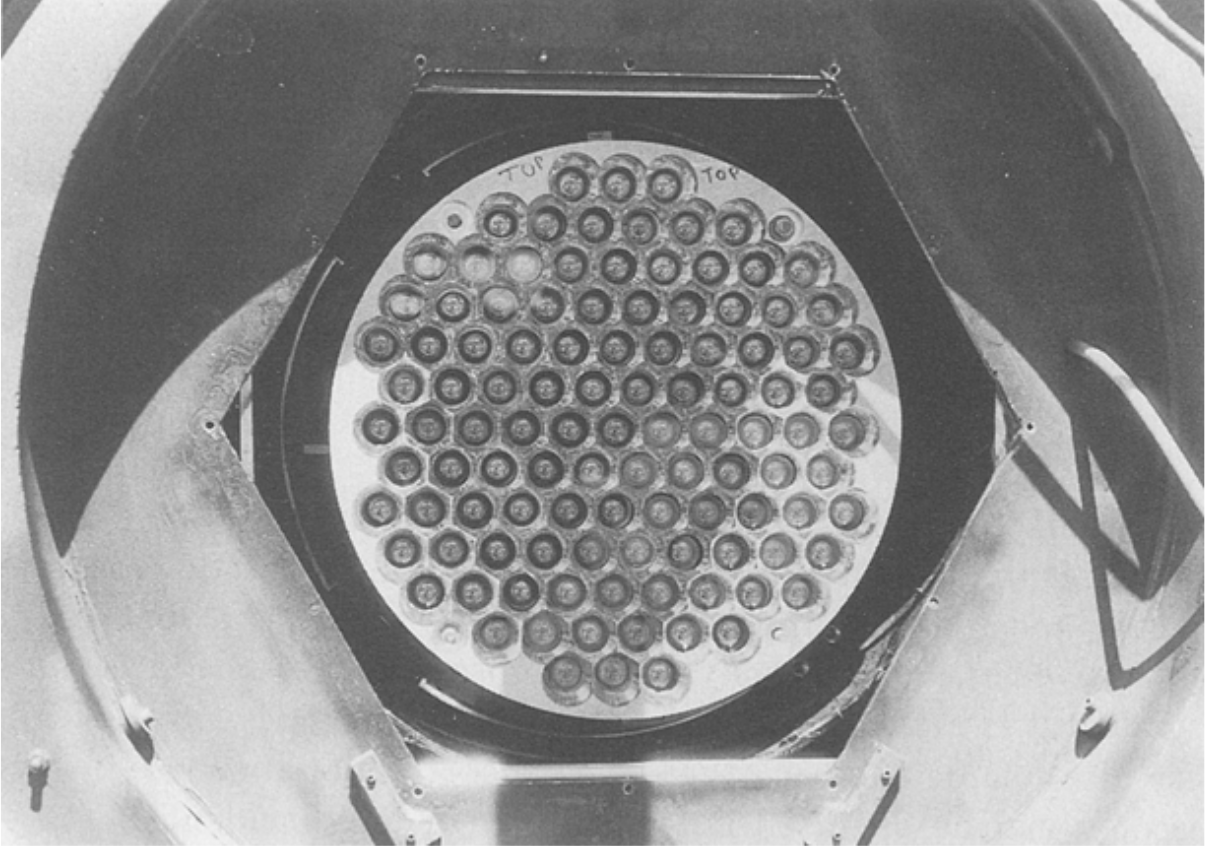
\includegraphics[width=0.8\textwidth]{images/whipple_cam.png}
    \caption{Picture of the upgraded camera of the Whipple telescope, installed in 1988 \cite{Cawley1995}.}  % not the best source
    \label{fig:whipple_cam}
\end{figure}

The shower images in combination with better computer simulations allowed for 
superior background rejection based on the  hillas-parameters.
1989 had the telescope observing the Crab Nebula with 9$\sigma$ 
\cite{1989ApJ...342..379W}.


Another big experiment of the time was the HEGRA experiment, an array consisting 
of 37 \SI{1}{\meter^2} scintillation detectors \cite{ALLKOFER1990345} in the first stage.
While at this stage not technically an IACT-experiment, later upgrade plans
brought multiple \SI{8.5}{\meter^2} diameter telescopes, starting with the first 
telescope in 1985 \cite{DAUM19971}.
While each telescope does not look too impressive on its own,
the so called HEGRA-IACT array made for a great use of the stereo principle,
marking the transition to the third generation of IACTs.


\subsection{The third generation}

Towards the end of the 1990s several third generation telescopes were
proposed:
H.E.S.S and MAGIC, deriving from parts of the HEGRA collaboration, 
VERITAS from Whipple and the no longer operating CANGAROO from Adelaide and 
several japanese universities \cite{HILLAS201319}.
All of these were designed as stereoscopic imaging telescopes building on the progress made during the 
second generation with two experiments located on each the north and the south hemisphere.

\subsubsection{Major Atmospheric Gamma Imaging Telescopes (MAGIC)}
- jahre für phase 1 und 2 ergänzen
- location ergänzen

MAGIC is a experiment initially operating as single telescope with a second slightly improved 
telescope added later \cite{BAIXERAS2003247}.
Both telescopes have a 17m diameter, 964 elements mirror making MAGIC-I the biggest 
telescope at its time.

In the second phase MAGIC operates in the energy range from \SI{30}{\giga\eV}
up to \SI{1}{\TeV} (cite website?).

The DISP-method for the reconstruction of the event arrival direction 
was significantly improved by including timing information and showed better 
results for stereoscopy than the simple crossing of the main shower axis \cite{ALEKSIC2012345}.

A specialty of the MAGIC experiment lies in its ability to 
perform fast skews and thus react to gamma ray bursts after they have been observed 
by satellite experiments \cite{2003ICRC....5.2943B}.

This enabled the recent observation of the very first \si{\TeV}
gamma ray burst observed with IACTs \cite{collaboration2019teraelectronvolt}.


\subsubsection{High Energy Stereoscopic System (HESS)}

The HESS experiment, located in Namibia,  consists of five telescopes.

A similar distinction in phase I and phase II can be taken with 
HESS phase I consisting of four \SI{13}{\meter} diameter telescopes,
arranged at the edge of a square of \SI{120}{\meter} long sides \cite{HINTON2004331}.
These operated from 2004 to 2012 when the experiment went into phase II.

Phase II brought the fifth, larger telescope with the aim to lower the energy threshold
further \cite{vincent2005hess}. This \SI{24}{\meter} telescope was placed in the middle of the other
telescopes.

- besonderheiten und entdeckungen

\subsubsection{Very Energetic Radiation Imaging Telescope Array System (VERITAS)}
VERITAS	was initially planned as a seven-telescope array, arranged in a diamond shape
\cite{WEEKES2020221}.
Each telescope covers a 3.5° FoV with a \SI{12}{\meter} diameter mirror and 
a 499 pixel PMT camera.


Eventually the collaboration settled 
with four telescopes. A relocation of telescope 1 in 2009 meant that the 
experiment made better use of the given area and its four telescopes \cite{2009arXiv0912.3841P}.
The old and new layout can be seen in figure \ref{fig:veritas_erlocation}

\begin{figure}
	\center
	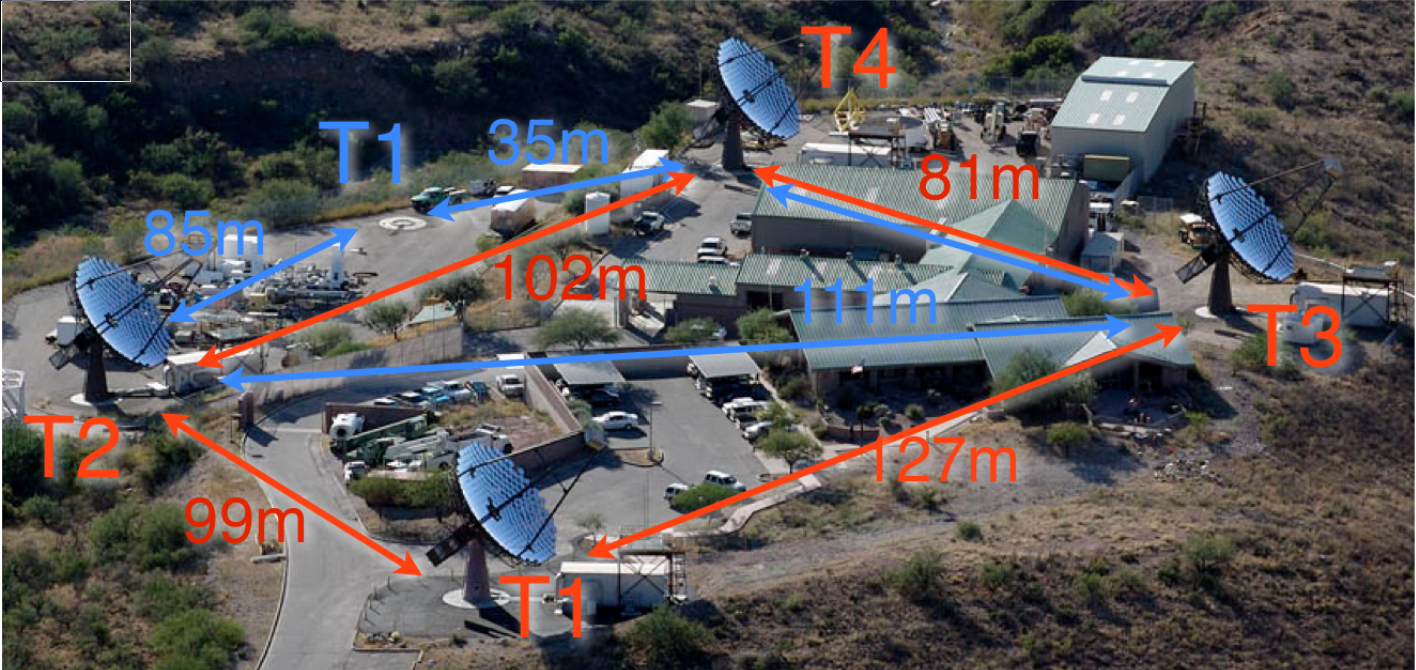
\includegraphics[width=.8\textwidth]{images/veritas_relocation.png}
	\caption{The VERITAS array layout after relocation of the first 
		telescope. The distances between the telescopes are 
	highlighted for the old(blue) and the new(red) array \cite{2009arXiv0912.3841P}.}
	\label{fig:veritas_relocation}
\end{figure}

Like MAGIC, VERITAS makes use of the DISP-method, especially at large zenith angles 
\cite{2015ICRC...34..771P}.



\section{Next to come: The Cherenkov Telescope Array (CTA)}
The Cherenkov Telescope Array aims to be the next generation of IACT experiments.
With two sites of operation, one for each hemisphere, and a number of 
telescopes proposed, CTA is going to expand on the findings of the third 
generation of telescopes.

Like HESS in phase II, the CTA arrays are going to consist of different sized telescopes, namely
the large-sized telescope (LST, \SI{23}{\meter}), 
the medium-sized telescope (MST, \SI{12}{\meter}) 
and the small-sized telescope (SST, \SI{4.3}{\meter}).

Extensive monte carlo simulations have been performed to find optimal array arrangements
\cite{BERNLOHR2013171}.

The currently planned layouts at LaPalma and in Namibia are shown in 
\ref{fig:cta_layout}

\begin{figure}
	\center
	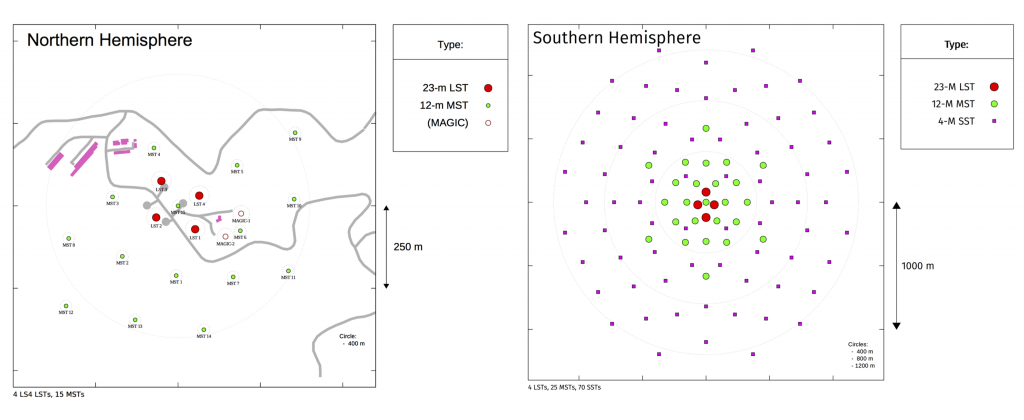
\includegraphics[width=0.8\textwidth]{images/cta_layout.png}
	\caption{The planned layouts \cite{cta_web}}
	\label{fig:cta_layout}
\end{figure}


\subsection{LST}
groß, niedrige energie, ...

\begin{figure}
	\center
	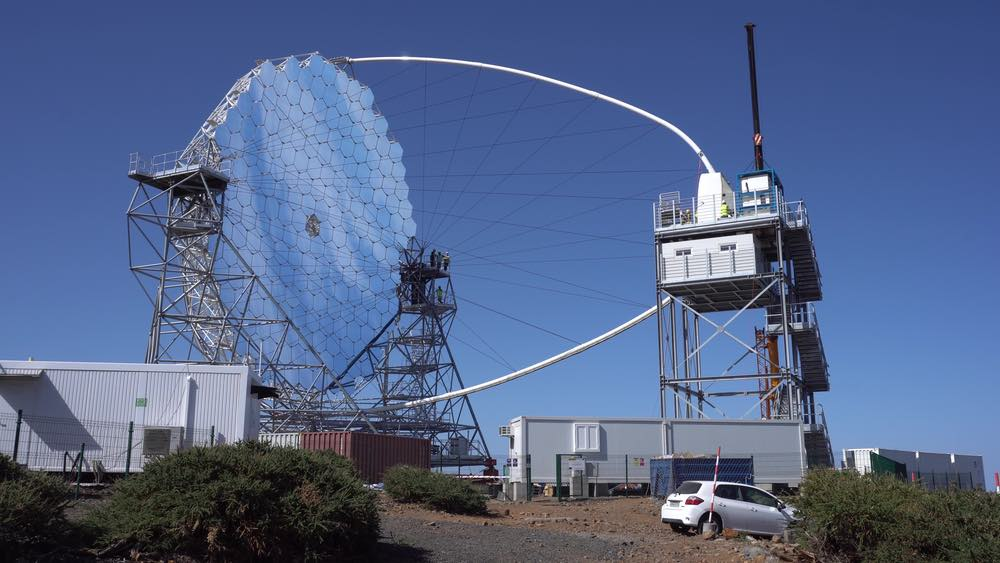
\includegraphics[width=.8\textwidth]{images/lst.jpeg}
	\caption{lst \cite{cta_web}}
	\label{fig:lst}
\end{figure}

\subsection{MST}
mittel, mittel energie, ...

\begin{figure}
	\center
	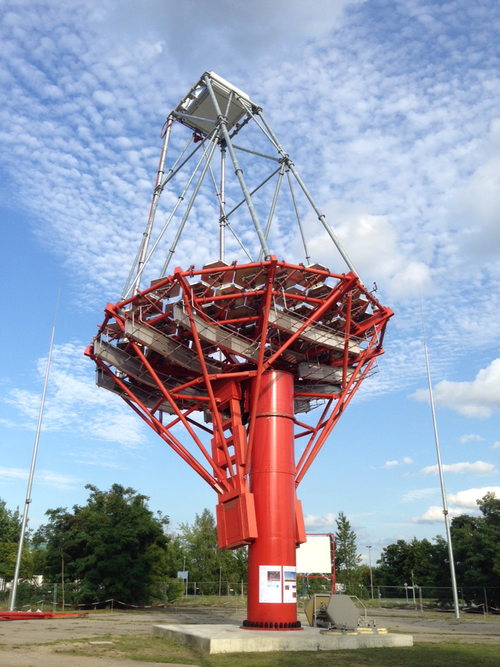
\includegraphics[width=.8\textwidth]{images/mst.png}
	\caption{mst \cite{cta_web}}
	\label{fig:mst}
\end{figure}

\subsection{SST}
klein, doppel mirror, viele, hohe energien

\begin{figure}
	\center
	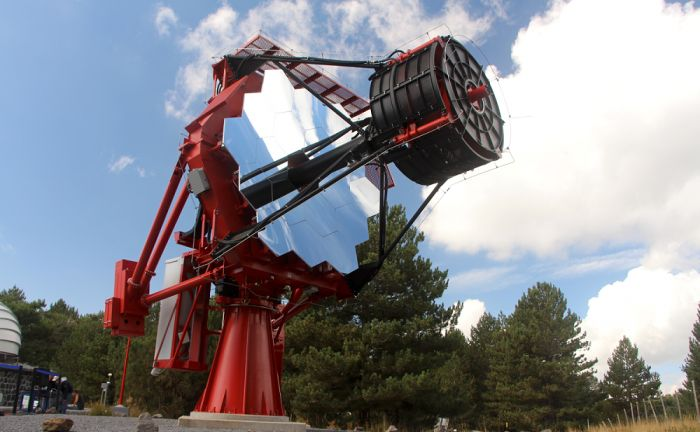
\includegraphics[width=.8\textwidth]{images/sst.jpg}
	\caption{sst \cite{cta_web}}
	\label{fig:sst}
\end{figure}



\subsection{Open observatory}
hier dann von \cite{actis2011design} zitieren.

% bis vlt seite 15-25
